\documentclass[journal,12pt,onecolumn]{IEEEtran}
\usepackage{cite}
\usepackage{amsmath,amssymb,amsfonts,amsthm}
\usepackage{algorithmic}
\usepackage{graphicx}
\graphicspath{{./figs/}}
\usepackage{textcomp}
\usepackage{xcolor}
\usepackage{txfonts}
\usepackage{listings}
\usepackage{enumitem}
\usepackage{mathtools}
\usepackage{gensymb}
\usepackage{comment}
\usepackage{caption}
\usepackage[breaklinks=true]{hyperref}
\usepackage{tkz-euclide} 
\usepackage{listings}
\usepackage{gvv}                                           
\usepackage{xparse}
\usepackage{color}                                            
\usepackage{array}                                            
\usepackage{longtable}                                       
\usepackage{calc}                                             
\usepackage{multirow}
\usepackage{multicol}
\usepackage{hhline}                                           
\usepackage{ifthen}                                           
\usepackage{lscape}
\usepackage{tabularx}
\usepackage{array}
\usepackage{float}
\usepackage[margin=1in]{geometry}
\usepackage{fancyhdr}
\usepackage{chemfig}
\usepackage{multicol}
 \usepackage{amsmath}
\usepackage{enumitem}
\usepackage{array}
\usepackage{titlesec}
\usepackage{tabularx} 
\usepackage{amsmath, amssymb}
\usepackage{extarrows}
\usepackage{chemarr}
\usepackage[utf8]{inputenc}
\usepackage{chemmacros} 
\usepackage{graphicx}
\chemsetup{modules={reactions}} 


% Header settings
\pagestyle{fancy}
\fancyhf{}
\fancyhead[L]{\textit{2008}}
\fancyhead[R]{\textbf{LIFE SOURCES--XL}}
\renewcommand{\headrulewidth}{0.4pt}

\begin{document}

\section*{\centering J : CHEMISTRY (Compulsory)}
\fbox{%
  \parbox{15cm}{
    \textbf{Useful data for Section J: Chemistry} \\
    $\ln 2 = 0.693$; $\ln 10 = 2.303$; $R = 8.314 \, J\,K^{-1}\,mol^{-1} = 0.083\, L\,bar\,K^{-1}\,mol^{-1}$; \\
    $K_{sp} (\mathrm{AgCl}) = 1.8 \times 10^{-10}$, $K_{sp} (\mathrm{AgI}) = 8.3 \times 10^{-17}$; Trouton's constant $= 85$
  }
}

\noindent\textbf{Q. 1 -- Q. 6 carry one mark each.}

\begin{enumerate}
    \item Which of the following will \textbf{NOT} conduct electricity?  
    \begin{multicols}{2}
    \begin{enumerate}[label=(\Alph*)]
        \item Solid metallic Na  
        \item Solid NaCl  
        \item Aqueous NaCl  
        \item Fused NaCl  
    \end{enumerate}
    \end{multicols}

    \item The region in which the following spectral lines are observed is \\
    P. Lyman series \hspace{1cm} Q. Balmer series \hspace{1cm} R. Paschen series  
    \begin{multicols}{2}
    \begin{enumerate}[label=(\Alph*)]
        \item P -- UV, Q -- UV/Vis, R -- IR  
        \item P -- UV/Vis, Q -- UV, R -- IR  
        \item P -- IR, Q -- UV, R -- Vis/IR  
        \item P -- UV, Q -- IR, R -- UV/Vis  
    \end{enumerate}
    \end{multicols}

    \item The pH of a $10^{-8}$ molar hydrochloric acid solution is  
    \begin{multicols}{2}
    \begin{enumerate}[label=(\Alph*)]
        \item exactly 8  
        \item between 7 and 8  
        \item exactly 7  
        \item between 6 and 7  
    \end{enumerate}
    \end{multicols}

    \item The plot of concentration of A against time is a straight line with negative slope for the reaction:  
    \[
    A \longrightarrow \text{products}
    \]  
    The order of the reaction is  
    \begin{multicols}{2}
    \begin{enumerate}[label=(\Alph*)]
        \item $-1$  
        \item 0  
        \item 1  
        \item 2  
    \end{enumerate}
    \end{multicols}

    \item Among the following four amines, which one is \textbf{least basic} in aqueous solution?  
    \begin{multicols}{2}
    \begin{enumerate}[label=(\Alph*)]
        \item CH$_3$NH$_2$  
        \item (CH$_3$)$_2$NH  
        \item (CH$_3$)$_3$N  
        \item CH$_3$NHCH$_3$  
    \end{enumerate}
    \end{multicols}

    \item Which of the following acids is used for the preparation of cyclohexene from cyclohexanol?  
    \begin{multicols}{2}
    \begin{enumerate}[label=(\Alph*)]
        \item Conc. HNO$_3$  
        \item 48\% HBr  
        \item 85\% H$_3$PO$_4$  
        \item (COOH)$_2$  
    \end{enumerate}
    \end{multicols}
\end{enumerate}

\noindent\textbf{Q. 7 to Q. 8 carry two marks each.}

\begin{enumerate}
\setcounter{enumi}{6}
    \item An aqueous mixture solution is prepared which contains 0.1 M of KCl and 0.1 M KI. To this solution, a drop of 0.01 M aqueous solution of AgNO$_3$ is added. Which of the following statement is correct?  
    \begin{multicols}{2}
    \begin{enumerate}[label=(\Alph*)]
        \item A precipitate forms which is primarily AgI.  
        \item A precipitate forms which is primarily AgCl.  
        \item A precipitate forms which has equimolar amounts of AgCl and AgI.  
        \item There will be no precipitation, as there is no common ion between potassium and silver salts.  
    \end{enumerate}
    \end{multicols}

    \item 1 g L$^{-1}$ solution of a protein exerts an osmotic pressure of $8.3 \times 10^{-3}$ bar at 300 K. Calculate the molar mass of the protein.  
    \begin{multicols}{2}
    \begin{enumerate}[label=(\Alph*)]
        \item 2490 g mol$^{-1}$  
        \item 3000 g mol$^{-1}$  
        \item 4578 g mol$^{-1}$  
        \item 6100 g mol$^{-1}$  
    \end{enumerate}
    \end{multicols}
    \item An electrochemical cell of the following representation was found to be a galvanic cell, where ‘A’ and ‘B’ represent different metals.  
    \[
    A (s) \,|\, A^{2+} (aq) \, 1\,M \,||\, B^{2+} (aq) \, 1\,M \,|\, B(s)
    \]  
    Which of the following statements with respect to the cell is correct?  
    \begin{multicols}{2}
    \begin{enumerate}[label=(\Alph*)]
        \item The cell converts electrical energy to chemical energy spontaneously.
        \item The cell uses electrical energy to deposit ‘A’ and dissolve ‘B’ spontaneously.
        \item (A$^{2+}$/A) is a stronger reducing agent than (B$^{2+}$/B).
        \item (A$^{2+}$/A) is a stronger oxidizing agent than (B$^{2+}$/B).
    \end{enumerate}
    \end{multicols}

    \item For a first order reaction at a particular temperature, the half-life was found to be (100 ln2) seconds. The specific rate constant of the reaction is  
    \begin{multicols}{4}
    \begin{enumerate}[label=(\Alph*)]
        \item 0.01 s$^{-1}$
        \item 100 s$^{-1}$
        \item 230 s$^{-1}$
        \item 693 s$^{-1}$
    \end{enumerate}
    \end{multicols}

    \item Liquid bromine boils at 59$^\circ$C. Assuming it to be a normal liquid, which of the following gives its standard molar enthalpy of vaporization?  
    \begin{multicols}{4}
    \begin{enumerate}[label=(\Alph*)]
        \item (8.314 $\times$ 332) J mol$^{-1}$
        \item (85 $\times$ 332) J mol$^{-1}$
        \item (332 / 85) J mol$^{-1}$
        \item (332 / 8.314) J mol$^{-1}$
    \end{enumerate}
    \end{multicols}

    \item The limiting molar conductivities of some species are given in (S cm$^2$ mol$^{-1}$) units: \\
    $\Lambda^0$(HCl) = 425.9; $\Lambda^0$(NaCl) = 126.4; $\Lambda^0$(H$^+$) = 349.6 \\
    Find the limiting molar conductivity of Na$^+$ ion.  
    \begin{multicols}{4}
    \begin{enumerate}[label=(\Alph*)]
        \item 50.1
        \item 76.3
        \item 299.5
        \item 476.0
    \end{enumerate}
    \end{multicols}

    \item The reactivity order for nitration of benzene, chlorobenzene, phenol and nitrobenzene is  
    \begin{multicols}{2}
    \begin{enumerate}[label=(\Alph*)]
        \item Benzene $>$ Chlorobenzene $>$ Phenol $>$ Nitrobenzene
        \item Phenol $>$ Benzene $>$ Chlorobenzene $>$ Nitrobenzene
        \item Nitrobenzene $>$ Phenol $>$ Chlorobenzene $>$ Benzene
        \item Phenol $>$ Chlorobenzene $>$ Benzene $>$ Nitrobenzene
    \end{enumerate}
    \end{multicols}

\({\chemfig{*6(------)=CH_2}} 
\underset{\text{$CCl_{4}$, benzoyl peroxide}}{\overset{\text{NBS}}{\longrightarrow}} 
\)
 \item The major product in the above reaction is:
  \begin{enumerate}[label=(\Alph*)]
   
    \item{\chemfig{*6(------)-CH_2Br}}
    \item{\chemfig{*6(-----(=CH_2)-)-[:60,0.75]Br}}
    \item{\chemfig{*6(------)-CH_2Br}}
    \item{\chemfig{*6(---(-CH_2Br)-(-Br)---)}}
 \end{enumerate}

    \item When a compound (M) is slowly heated with chloroform in alcoholic KOH solution, it produces an offensive smell. The compound M is  
    \begin{multicols}{4}
    \begin{enumerate}[label=(\Alph*)]
        \item N,N-Diethylamine
        \item Diethylamine
        \item Ethylamine
        \item Triethylamine
    \end{enumerate}
    \end{multicols}

\item Which one of the following will lactonize in presence of acid?
\begin{multicols}{4}
\begin{enumerate}[label=(\Alph*)]
 \item\scalebox{0.4}{\chemfig{
*6(
  -[:0](<..COOH)  
  -[:60]
  -[:120](<:OH)
  -[:180]
  -[:240]
  -[:300]
)
}}
 \item\scalebox{0.4}{\chemfig{
*6(
  -[:0](<..COOH)  
  -[:60]
  -[:120](<..OH)
  -[:180]
  -[:240]
  -[:300]
)
}}
 \item\scalebox{0.4}{\chemfig{
*6(
  -[:0](<..OH)  
  -[:60]
  -[:120]
  -[:180](<:COOH)
  -[:240]
  -[:300]
)
}}
 \item\scalebox{0.4}{\chemfig{
*6(
  -[:0](<..OH)  
  -[:60]
  -[:120](<..CH_3)
  -[:180](<:COOH)
  -[:240]
  -[:300]
)
}}
\end{enumerate}
\end{multicols}

\item The major condensation product in the reaction of benzaldehyde with excess amount of acetone in presence of dilute NaOH solution is
\begin{multicols}{2}
\begin{enumerate}[label=(\Alph*)]
\item\scalebox{0.7}{\chemfig{
C_6H_5-CH=CH-C([::60]=O)-[::-60]CH_3
}}

  \item  \scalebox{0.7}{\chemfig{
C_6H_5-CH=CH-C([::60]=O)-[::-60]CH=CH-C_6H_5
}}
  \item[(C)]\scalebox{0.7}{\chemfig{
CH_3-C(-[::60]CH_3)=CH-CH_2-C([::60]=O)-[::-60]CH_3
}
}
  \item    \scalebox{0.7}{\chemfig{
C_6H_5-CH(-[::60]OH)-CH_2-C([::60]=O)-[::-60]CH_3
}}
\end{enumerate}
\end{multicols}

\item Ammonia gas can be dried over
\begin{multicols}{4}
\begin{enumerate}[label=(\Alph*)]
\item conc. H\textsubscript{2}SO\textsubscript{4}
\item anhydrous P\textsubscript{2}O\textsubscript{5}
\item anhydrous CaO
\item anhydrous CaCl\textsubscript{2}
\end{enumerate}
\end{multicols}

\item Which of the following molecules will have zero dipole moment?\\
H\textsubscript{2}O, SiCl\textsubscript{4}, CO\textsubscript{2}, NH\textsubscript{3}, BF\textsubscript{3}
\begin{multicols}{2}
\begin{enumerate}[label=(\Alph*)]
\item H\textsubscript{2}O, SiCl\textsubscript{4}, BF\textsubscript{3}
\item CO\textsubscript{2}, NH\textsubscript{3}, SiCl\textsubscript{4}
\item H\textsubscript{2}O, NH\textsubscript{3}, BF\textsubscript{3}
\item CO\textsubscript{2}, BF\textsubscript{3}, SiCl\textsubscript{4}
\end{enumerate}
\end{multicols}

\item Which of the following pairs of complexes will NOT show any ligand field d–d transitions?
\begin{multicols}{2}
\begin{enumerate}
  \item[(A)] K\textsubscript{4}[Fe(CN)\textsubscript{6}], [Ni(H\textsubscript{2}O)\textsubscript{6}](NH\textsubscript{3})\textsubscript{2}SO\textsubscript{4}
  \item[(B)] [Cu(CH\textsubscript{3}CN)\textsubscript{4}]Cl, Na[CoCl\textsubscript{4}(CN)\textsubscript{4}]
  \item[(C)] [Cu(CH\textsubscript{3}CN)\textsubscript{4}]Cl, [Zn(NH\textsubscript{3})\textsubscript{4}Cl\textsubscript{2}]
  \item[(D)] [Cu(H\textsubscript{2}O)\textsubscript{6}](NH\textsubscript{3})\textsubscript{2}Cl\textsubscript{2}, [Zn(H\textsubscript{2}O)\textsubscript{4}(NH\textsubscript{3})\textsubscript{2}]SO\textsubscript{4}
\end{enumerate}
\end{multicols}


\item Which of the following substances will produce acidic oxides when burnt in excess air?\\
Sodium (P), Sulfur (Q) and Methane (R)
\begin{multicols}{2}
\begin{enumerate}[label=(\Alph*)]
\item All three
\item Both Q and R
\item Only Q
\item Both P and R
\end{enumerate}
\end{multicols}

\item In the ring test for nitrate ion, the brown color is due to the formation of
\begin{multicols}{2}
\begin{enumerate}[label=(\Alph*)]
 \item[(A)] [Fe(H\textsubscript{2}O)\textsubscript{5}(NO)]SO\textsubscript{4}
  \item[(B)] [Fe(H\textsubscript{2}O)\textsubscript{5}(NO\textsubscript{2})]SO\textsubscript{4}
  \item[(C)] [Fe(H\textsubscript{2}O)\textsubscript{5}(NO\textsubscript{3})]SO\textsubscript{4}
  \item[(D)] [Fe(H\textsubscript{2}O)\textsubscript{5}(NO\textsubscript{3})]SO\textsubscript{4}
\end{enumerate}
\end{multicols}
\item The appropriate reagent (O) required for this transformation is
\begin{multicols}{2}
\begin{enumerate}[label=(\Alph*)]
\item KOH / EtOH
\item NaOMe / MeOH
\item NaI / Acetone
\item NaNH$_2$
\end{enumerate}
\end{multicols}

\item The alkene will be produced as

\begin{enumerate}[label=(\Alph*)]
\item P exclusively since it is going through E2 mechanism
\item Q exclusively since it is going through E2 mechanism
\item Equal amount of P and Q since it is going through E1 mechanism
\item P as major amount since it is going through E1cB mechanism
\end{enumerate}



\noindent\textbf{Linked Answer Questions: Q.25 to Q.28 carry two marks each.}

\noindent \textbf{Statement for Linked Answer Questions 25 and 26:} 

CuSO$_4$ solution when treated with aqueous alkali (W) forms a blue precipitate (X), which dissolves on addition of excess W. Another aqueous alkali (Y) precipitates blue solid (Z) when reacted with CuSO$_4$, but the blue precipitate (Z) does not dissolve with excess alkali (Y).


\item Identify W and X
\begin{multicols}{2}
\begin{enumerate}[label=(\Alph*)]
\item NH$_4$OH and Cu(OH)$_2\cdot$CuSO$_4$
\item NH$_4$OH and Cu(OH)$_2$
\item NaOH and Cu(OH)$_2\cdot$CuSO$_4$
\item NaOH and Cu(OH)$_2$
\end{enumerate}
\end{multicols}

\item Identify Y and Z
\begin{multicols}{2}
\begin{enumerate}[label=(\Alph*)]
\item NH$_4$OH and Cu(OH)$_2\cdot$CuSO$_4$
\item NH$_4$OH and Cu(OH)$_2$
\item NaOH and Cu(OH)$_2\cdot$CuSO$_4$
\item NaOH and Cu(OH)$_2$
\end{enumerate}
\end{multicols}


\noindent \textbf{Statement for Linked Answer Questions 27 and 28:} 

For a first order reversible reaction
\[
A \xrightleftharpoons[k_b]{k_f} B
\]
at a temperature T, the standard molar free energy ($\Delta G^\circ$) is equal to $-2.303RT$, and the rate constant of forward reaction ($k_f$) is $1 \times 10^{-3}$ s$^{-1}$.

\item The equilibrium constant of the reaction is
\begin{multicols}{4}
\begin{enumerate}[label=(\Alph*)]
\item 23.03
\item 19.09
\item 10
\item 1
\end{enumerate}
\end{multicols}

\item The rate constant of the backward reaction ($k_b$) is
\begin{multicols}{4}
\begin{enumerate}[label=(\Alph*)]
\item $5.26 \times 10^{-5}$ s$^{-1}$
\item $1 \times 10^{-2}$ s$^{-1}$
\item $4.35 \times 10^{-5}$ s$^{-1}$
\item $1 \times 10^{-4}$ s$^{-1}$
\end{enumerate}
\end{multicols}
\end{enumerate}
\begin{center}
    \textbf{END OF SECTION -J}
\end{center}
\newpage
\section*{\centering K: BIOCHEMISTRY}

\noindent \textbf{Q.1 -- Q.6 carry one mark each.}

\begin{enumerate}

\item Which of the following inhibitor uncouples electron transport and oxidative phosphorylation?
\begin{multicols}{4}
\begin{enumerate}[label=(\Alph*)]
\item Azide
\item Dinitrophenol
\item Oligomycin
\item Rotenone
\end{enumerate}
\end{multicols}

\item The catalytic efficiency of an enzyme is represented by
\begin{multicols}{4}
\begin{enumerate}[label=(\Alph*)]
\item $V_{\text{max}}$
\item $K_M$
\item $k_{\text{cat}}$
\item $k_{\text{cat}}/K_M$
\end{enumerate}
\end{multicols}

\item Which of the following activate protein kinase C?
\begin{multicols}{4}
\begin{enumerate}[label=(\Alph*)]
\item Inositol 1,4,5-trisphosphate
\item Cyclic AMP
\item Inositol
\item Diacylglycerol
\end{enumerate}
\end{multicols}

\item Transcription initiation sites can be determined by
\begin{multicols}{4}
\begin{enumerate}[label=(\Alph*)]
\item Footprinting
\item Northern blotting
\item Primer extension
\item Nick translation
\end{enumerate}
\end{multicols}

\item One common feature between B and T cells is that
\begin{multicols}{2}
\begin{enumerate}[label=(\Alph*)]
\item both cells produce antibodies
\item both cells possess MHC class II
\item both B cell receptor and T cell receptor undergo rearrangement
\item both cells can produce cytokines
\end{enumerate}
\end{multicols}

\item In hybridoma technology, the myeloma cells used
\begin{multicols}{2}
\begin{enumerate}[label=(\Alph*)]
\item lack HGPRTase
\item lack the ability to produce Ig
\item lack both HGPRTase and ability to produce Ig
\item lack thymidine kinase
\end{enumerate}
\end{multicols}


\noindent \textbf{Q.7 to Q.24 carry two marks each.}


\item Match the function in Column I with organelle in Column II

\noindent
\begin{tabular}{p{6cm} p{6cm}}
\textbf{Column I} & \textbf{Column II} \\
(P) Protein synthesis & (1) Endoplasmic reticulum \\
(Q) Protein degradation & (2) Golgi body \\
(R) Protein glycosylation & (3) Lysosome \\
& (4) Peroxisome
\end{tabular}

\begin{multicols}{2}
\begin{enumerate}[label=(\Alph*)]
\item P-3,\ Q-2,\ R-1
\item  P-1,\ Q-3,\ R-2
\item   P-1,\ Q-4,\ R-3
\item    P-4,\ Q-1,\ R-2
\end{enumerate}
\end{multicols}

\item Match the polysaccharides in Column I with their constituent monosaccharide in Column II

\noindent
\begin{tabular}{p{6cm} p{6cm}}
\textbf{Column I} & \textbf{Column II} \\
(P) Chitin & (1) D-Glucose \\
(Q) Hemicellulose & (2) N-Acetyl glucosamine \\
(R) Glycogen & (3) D-Xylose \\
& (4) D-Galactose
\end{tabular}

\begin{multicols}{2}
\begin{enumerate}[label=(\Alph*)]
\item P-1,\ Q-3,\ R-4
\item  P-2,\ Q-1,\ R-3
\item   P-4,\ Q-2,\ R-1
\item    P-2,\ Q-3,\ R-1
\end{enumerate}
\end{multicols}
\item The $T_m$ of phosphatidyl choline A is higher than $T_m$ of phosphatidyl choline B because
\begin{multicols}{2}
\begin{enumerate}[label=(\Alph*)]
\item has shorter chain fatty acid and more unsaturated fatty acid than B
\item has longer chain fatty acid and more saturated fatty acid than B
\item has shorter chain fatty acid than B
\item has more \textit{cis}-unsaturated fatty acid than B
\end{enumerate}
\end{multicols}

\item A mixture of proteins namely P, Q, R and S having molecular mass 50, 80, 120, and 150 KDa is applied on the Sephadex-G 200 column. The order of their elution will be
\begin{multicols}{2}
\begin{enumerate}[label=(\Alph*)]
\item P, Q, R, S
\item S, R, Q, P
\item Q, P, R, S
\item P, Q, S, R
\end{enumerate}
\end{multicols}

\item Match the transition state or chemical entity of each enzyme that is responsible for their catalytic function

\noindent
\begin{tabular}{p{5cm} p{5cm}}
\textbf{Column I} & \textbf{Column II} \\
(P) Ribonuclease & (1) Oxyanion \\
(Q) Lysozyme & (2) Pentacovalent phosphorus \\
(R) Chymotrypsin & (3) Carbonium ion \\
(S) Carboxypeptidase & (4) Mixed anhydride
\end{tabular}

\begin{multicols}{2}
\begin{enumerate}[label=(\Alph*)]
\item P-3,\ Q-2,\ R-1,\ S-4
\item  P-2,\ Q-3,\ R-1,\ S-4
\item   P-2,\ Q-1,\ R-3,\ S-4
\item    P-4,\ Q-3,\ R-2,\ S-1
\end{enumerate}
\end{multicols}

\item Match the function of following cofactors

\noindent
\begin{tabular}{p{6cm} p{7cm}}
\textbf{Column I} & \textbf{Column II} \\
(P) Thiamine pyrophosphate & (1) Acyl group transfer \\
(Q) Coenzyme A & (2) Transfer of one carbon component \\
(R) Pyridoxal phosphate & (3) Group transfer to/from amino acid \\
(S) Tetrahydrofolate & (4) Aldehyde transfer
\end{tabular}

\begin{multicols}{2}
\begin{enumerate}[label=(\Alph*)]
\item P-4,\ Q-3,\ R-1,\ S-2
\item  P-4,\ Q-3,\ R-2,\ S-1
\item   P-4,\ Q-1,\ R-3,\ S-2
\item    P-3,\ Q-1,\ R-4,\ S-2
\end{enumerate}
\end{multicols}

\item Match the enzymes in Column I with their metabolic pathways in Column II

\noindent
\begin{tabular}{p{8cm} p{6cm}}
\textbf{Column I} & \textbf{Column II} \\
(P) Succinyl CoA synthetase & (1) $\beta$-Oxidation \\
(Q) Acyl CoA dehydrogenase & (2) Calvin cycle \\
(R) Transketolase & (3) Tricarboxylic acid cycle \\
(S) Ribulose 1,5-bisphosphate carboxylase & (4) Pentose phosphate pathway
\end{tabular}

\begin{multicols}{2}
\begin{enumerate}[label=(\Alph*)]
\item P-1,\ Q-3,\ R-4,\ S-2
\item  P-3,\ Q-1,\ R-2,\ S-4
\item   P-2,\ Q-4,\ R-1,\ S-3
\item    P-3,\ Q-1,\ R-4,\ S-2
\end{enumerate}
\end{multicols}
\item Glycolysis and gluconeogenesis are reciprocally coordinated. Which of the following will activate pyruvate carboxylase in gluconeogenesis?
\begin{multicols}{2}
\begin{enumerate}[label=(\Alph*)]
\item Acetyl CoA
\item Fructose 2,6-bisphosphate
\item ADP
\item ATP
\end{enumerate}
\end{multicols}

\item The atoms of pyrimidine ring are derived from  
(P) Carbamoyl phosphate \quad (Q) Inosine mono phosphate \quad (R) Aspartate \quad (S) Glutamate
\begin{multicols}{2}
\begin{enumerate}[label=(\Alph*)]
\item P, Q
\item P, R
\item P, S
\item Q, R
\end{enumerate}
\end{multicols}

\item Which of the following statements are true for steroid hormones?  
(P) increase the enzymatic activity of pre-existing target enzyme  
(Q) act at cell nucleus  
(R) interact with the plasma membrane receptors of target cells  
(S) form a complex with receptor and acts as transcriptional enhancers
\begin{multicols}{2}
\begin{enumerate}[label=(\Alph*)]
\item P, R
\item Q, S
\item P, Q
\item R, S
\end{enumerate}
\end{multicols}

\item Match the items on the left with the inhibitors on the right

\noindent
\begin{tabular}{p{5cm} p{5cm}}
\textbf{Column I} & \textbf{Column II} \\
(P) DNA polymerase $\alpha$ & (1) Phenyl methyl sulphonyl fluoride (PMSF) \\
(Q) RNA polymerase II & (2) Aphidicolin \\
(R) Serine protease & (3) $\alpha$-amanitin \\
 & (4) Actinomycin
\end{tabular}

\begin{multicols}{2}
\begin{enumerate}[label=(\Alph*)]
\item P-2,\ Q-3,\ R-1
\item P-3,\ Q-1,\ R-2
\item P-2,\ Q-1,\ R-2
\item P-1,\ Q-2,\ R-4
\end{enumerate}
\end{multicols}

\item A nucleic acid sample is resistant to digestion with $\lambda$ exonuclease. When heated it does not show typical melting curve of a linear double stranded DNA. On CsCl-ethidium bromide equilibrium density centrifugation it settles at the bottom of the centrifuge tube. The nucleic acid is
\begin{multicols}{2}
\begin{enumerate}[label=(\Alph*)]
\item ccc pBR322
\item Bacteriophage P22 DNA
\item tRNA
\item RFII M13 DNA
\end{enumerate}
\end{multicols}

\item The following 4 different solutions are prepared by mixing the components of electron transport chain. Which among them is expected to cause a net transfer of electrons to cytochrome $c$?
\begin{multicols}{2}
\begin{enumerate}[label=(\Alph*)]
\item Reduced ubiquinone and reduced cytochrome $c$
\item Reduced ubiquinone, cytochrome $b-c_1$ complex and reduced cytochrome $c$
\item Oxidized ubiquinone and oxidized cytochrome $c$
\item Reduced ubiquinone, cytochrome $b-c_1$ complex and oxidized cytochrome $c$
\end{enumerate}
\end{multicols}

\item Nucleated cells tend to be more resistant to complement mediated lysis than RBC because
\begin{multicols}{2}
\begin{enumerate}[label=(\Alph*)]
\item many nucleated cells can endocytose the membrane attack complex
\item membrane attack complex cannot get inserted in the nucleated cell membrane
\item membrane attack complex can get inactivated by the nucleated cells
\item membrane attack complex get inactivated hence cannot get inserted in the nucleated cell membrane
\end{enumerate}
\end{multicols}

\item In a fluorescein labeled antibody to $\mu$ heavy chain and rhodamine labeled antibody to $\delta$ heavy chain, the fluorescent antibody staining pattern of the progenitor B cells (Pro-B cells) will be
\begin{multicols}{2}
\begin{enumerate}[label=(\Alph*)]
\item anti-$\mu$ staining in cytoplasm and on membrane
\item anti-$\mu$ and anti-$\delta$ staining in cytoplasm and on membrane
\item no cytoplasmic or membrane staining with either anti-$\mu$ or anti-$\delta$ antibody
\item anti-$\mu$ staining on membrane
\end{enumerate}
\end{multicols}
\item Serum IgM cannot activate the complement by itself because
\begin{multicols}{2}
\begin{enumerate}[label=(\Alph*)]
\item it does not have complement binding site
\item it is planar in which complement binding sites in the Fc region are not accessible
\item it gets degraded and hence unable to activate the complement
\item it needs metal ions to activate complement
\end{enumerate}
\end{multicols}
\noindent\textbf{Common Data Questions}

\noindent \textbf{Common Data for Questions 23 and 24:} 

A \textit{Caenorhabditis} contig for one region of chromosome 2 contains contiguous locations marked 1, 2, 3, 4, 5, 6, 7, 8 and 9. Cosmid clones a, b, c, d and e overlap the locations 2-4, 3-5, 4-6, 5-8, 8-9 respectively. A cloned pBR322-x hybridize to cosmids b, c and d and pUC18-y hybridize to cosmids d and e.

\item The approximate locations of x and y are
\begin{multicols}{2}
\begin{enumerate}[label=(\Alph*)]
\item 4 and 7
\item 5 and 8
\item 4 and 8
\item 5 and 7
\end{enumerate}
\end{multicols}

\item Both pBR322-x and pUC18-y will hybridize to cosmids
\begin{multicols}{2}
\begin{enumerate}[label=(\Alph*)]
\item b
\item d
\item e
\item c
\end{enumerate}
\end{multicols}

\noindent\textbf{Linked Answer Questions: Q.25 to Q.28 carry two marks each.}

\noindent\textbf {Statement for Linked Answer Questions 25 and 26:}

In animal cells concentration of sodium ions is higher outside the cell and less inside the cell, yet sodium does not enter the cells.


\item The cellular environment is maintained by generating a gradient and transporting the Na$^+$ outside the cell through
\begin{multicols}{2}
\begin{enumerate}[label=(\Alph*)]
\item diffusion process
\item passive transport via Na$^+$-K$^+$ pump
\item active transport via Na$^+$-K$^+$ pump
\item sodium ions not be transported
\end{enumerate}
\end{multicols}

\item Digitoxigenin, a cardiotonic steroid that inhibits ATPase when applied on extra cellular face of membrane, helps in accumulation of Ca$^{2+}$ inside the cardiac muscle cells by
\begin{multicols}{2}
\begin{enumerate}[label=(\Alph*)]
\item activating Na$^+$-K$^+$ pump and blocking Na$^+$-Ca$^{2+}$ exchanger
\item inhibiting Na$^+$-K$^+$ pump and blocking Na$^+$-Ca$^{2+}$ exchanger
\item having no effect on Na$^+$-K$^+$ pump
\item increasing passive diffusion
\end{enumerate}
\end{multicols}

\noindent \textbf{Statement for Linked Answer Questions 27 and 28:} \\
Nearly 46\% of 45S pre-rRNA is unstable. The remaining portion of it forms mature 5.8S, 18S and 28S rRNA having lengths 160 bases, 1.9 kb and 5.1 kb respectively. The content of pre rRNA per human genome is $7.8 \times 10^{-15}$ g.

\item The mol. wt. of 45S pre-rRNA is
\begin{multicols}{2}
\begin{enumerate}[label=(\Alph*)]
\item $2 \times 10^6$
\item $4.5 \times 10^5$
\item $4.5 \times 10^6$
\item $3.9 \times 10^7$
\end{enumerate}
\end{multicols}

\item The number of pre-rRNA genes per genome is approximately
\begin{multicols}{2}
\begin{enumerate}[label=(\Alph*)]
\item 10
\item 100
\item 1000
\item 10,000
\end{enumerate}
\end{multicols}

\end{enumerate}
\begin{center}
    \textbf{END OF SECTION -K}
\end{center}
\newpage
\section*{\centering L: BIOTECHNOLOGY}

\noindent\textbf{Q.1 – Q.6 carry one mark each.}

\begin{enumerate}
\item Diauxic pattern of biomass growth is associated with

(P) multiple lag phases  
(Q) sequential utilization of multiple substrates  
(R) simultaneous utilization of multiple substrates  
(S) absence of lag phase  

\begin{multicols}{2}
\begin{enumerate}[label=(\Alph*)]
    \item P, R
    \item P, Q
    \item R, S
    \item Q, S
\end{enumerate}
\end{multicols}

\item Zinc fingers are characteristics of
\begin{multicols}{2}
\begin{enumerate}[label=(\Alph*)]
    \item blood clotting proteins
    \item RNA chaperones
    \item DNA binding proteins
    \item lysosomal hydrolases
\end{enumerate}
\end{multicols}

\item Parthenogenetic embryos in plants are those which are formed by
\begin{multicols}{2}
\begin{enumerate}[label=(\Alph*)]
    \item unfertilized eggs
    \item fertilized eggs
    \item sporophytic cells
    \item male gametophyte
\end{enumerate}
\end{multicols}

\item Which one of the following is the growth factor used for growth of tissues and organs in plant tissue culture?
\begin{multicols}{2}
\begin{enumerate}[label=(\Alph*)]
    \item Cysteine
    \item Cytokinin
    \item Cytidylate
    \item Cyclic AMP
\end{enumerate}
\end{multicols}

\item Which of the following techniques is best suited for immobilizing an affinity ligand?
\begin{multicols}{2}
\begin{enumerate}[label=(\Alph*)]
    \item Physical adsorption
    \item Gel entrapment
    \item Cross-linking with a polymer
    \item Covalent linkage to a spacer arm
\end{enumerate}
\end{multicols}

\item Multiplication of genetically identical copies of a cultivar by asexual reproduction is known as
\begin{multicols}{2}
\begin{enumerate}[label=(\Alph*)]
    \item aclonal propagation
    \item vegetative propagation
    \item polyclonal propagation
    \item clonal propagation
\end{enumerate}
\end{multicols}
\end{enumerate}

\noindent\textbf{Q.7 to Q.24 carry two marks each.}

\begin{enumerate}
\setcounter{enumi}{6}
\item Identify the correct statements for the ‘HAT medium’
\begin{enumerate}[label=\Alph*:,start=16]
\item Includes drug aminopterin to block major pathway for synthesis of deoxyribonucleotides  
\item Hypoxanthine is precursor for thymidine  
\item Includes drug aminopterin to block major pathway for synthesis of polypeptides  
\item Cells can grow in presence of aminopterin only if they have enzymes thymidine kinase and hypoxanthine-guanine phosphoribosyl transferase
\end{enumerate}
\begin{multicols}{2}
\begin{enumerate}[label=(\Alph*)]
    \item P, Q
    \item P, S
    \item Q, S
    \item Q, S
\end{enumerate}
\end{multicols}
\item A DNA fragment of 4500 bp has to be tailed with dT residues by using dTTP and the enzyme ‘terminal transferase’. The stock solution of dTTP that is used as a substrate has a concentration of 150 $\mu$M. Ten $\mu$l of this stock solution is added to a total volume of 200 $\mu$l reaction. What will be the concentration of dTTP in the reaction?

\begin{multicols}{2}
\begin{enumerate}[label=(\Alph*)]
    \item 7.5 $\mu$M
    \item 75 $\mu$M
    \item 0.75 $\mu$M
    \item 0.075 $\mu$M
\end{enumerate}
\end{multicols}

\item Determine the correctness or otherwise of following \textbf{Assertion [a]} and \textbf{Reason [r]}  

\textbf{Assertion:} The enzymatic degradation of cell wall to obtain single cell called protoplast has helped immensely in developing somatic cell genetics in plants.  
\textbf{Reason:} In plants or animals, fusion of two cells must occur through the plasma membrane.

\begin{multicols}{2}
\begin{enumerate}[label=(\Alph*)]
    \item Both [a] and [r] are true and [r] is the correct reason for [a]
    \item Both [a] and [r] are true but [r] is not the correct reason for [a]
    \item [a] is true but [r] is false
    \item [a] is false but [r] is true
\end{enumerate}
\end{multicols}

\item In bioinformatics, the term ‘BLAST’ refers to
\begin{multicols}{2}
\begin{enumerate}[label=(\Alph*)]
    \item database retrieval tool
    \item computational tool for sequence homology searching and alignment
    \item computational tool to view genomic sequences
    \item computational tool to view protein structures
\end{enumerate}
\end{multicols}

\item Match the terms in Group 1 with their possible explanations in Group 2

\begin{center}
\begin{tabular}{ll}
\textbf{Group 1} & \textbf{Group 2} \\
P. Orthologs  & 1. A cell or an organism having foreign gene \\
Q. Paralogs   & 2. The complement of a protein expressed by a genome \\
R. Proteome   & 3. Genes from different species related to each other \\
S. Transgenic & 4. Genes from same species related to each other \\
\end{tabular}
\end{center}

\begin{multicols}{2}
\begin{enumerate}[label=(\Alph*)]
    \item P-2, Q-4, R-1, S-3
    \item P-4, Q-3, R-2, S-1
    \item P-3, Q-4, R-2, S-1
    \item P-1, Q-2, R-3, S-4
\end{enumerate}
\end{multicols}

\item Which of the following statements are true with respect to a special complex called ‘dicer’?

(P) It consists of deoxyribonuclease and DNA fragments  
(Q) It consists of ribonuclease and RNA fragments  
(R) It is involved in \textit{gene silencing}  
(S) It triggers apoptosis  

\begin{multicols}{2}
\begin{enumerate}[label=(\Alph*)]
    \item P, R
    \item Q, R
    \item P, S
    \item Q, S
\end{enumerate}
\end{multicols}

\item Some living cells (e.g., plant cell) have the capacity to give rise to whole organism. The term used to describe this property is
\begin{multicols}{2}
\begin{enumerate}[label=(\Alph*)]
    \item morphogenesis
    \item androgenesis
    \item totipotency
    \item organogenesis
\end{enumerate}
\end{multicols}
\item Match the items in group 1 with the terms given in group 2

\begin{center}
\begin{tabular}{ll}
\textbf{Group 1} & \textbf{Group 2} \\
P. \textit{Lactobacillus} and \textit{Bifidobacteria} & 1. Prebiotics \\
Q. Polychlorobenzenes (PCBs) & 2. Probiotics \\
R. Fructo-oligosaccharides & 3. Antibiotics \\
S. $\beta$-Lactams & 4. Xenobiotics \\
\end{tabular}
\end{center}

\begin{multicols}{2}
\begin{enumerate}[label=(\Alph*)]
    \item P-2, Q-4, R-1, S-3
    \item P-3, Q-4, R-1, S-2
    \item P-4, Q-1, R-2, S-3
    \item P-1, Q-3, R-4, S-2
\end{enumerate}
\end{multicols}

\item Match the coefficients in group 1 with their corresponding downstream processing steps given in group 2

\begin{center}
\begin{tabular}{ll}
\textbf{Group 1} & \textbf{Group 2} \\
P. Sedimentation coefficient & 1. Aqueous two-phase extraction \\
Q. Partition coefficient & 2. Ultrafiltration \\
R. Rejection coefficient & 3. Dialysis \\
S. Activity coefficient & 4. Centrifugation \\
\end{tabular}
\end{center}

\begin{multicols}{2}
\begin{enumerate}[label=(\Alph*)]
    \item P-3, Q-1, R-4, S-2
    \item P-2, Q-1, R-4, S-3
    \item P-4, Q-3, R-1, S-2
    \item P-4, Q-1, R-2, S-3
\end{enumerate}
\end{multicols}

\item Match the bioreactor components in group 1 with the most appropriate function given in group 2

\begin{center}
\begin{tabular}{ll}
\textbf{Group 1} & \textbf{Group 2} \\
P. Marine type impeller & 1. Recirculation of medium \\
Q. Draft tube & 2. Aeration of medium \\
R. Diaphragm valve & 3. Animal cell cultivation \\
S. Sparger & 4. Sterile operation \\
\end{tabular}
\end{center}

\begin{multicols}{2}
\begin{enumerate}[label=(\Alph*)]
    \item P-4, Q-2, R-1, S-3
    \item P-3, Q-1, R-4, S-2
    \item P-3, Q-4, R-2, S-1
    \item P-2, Q-1, R-4, S-3
\end{enumerate}
\end{multicols}

\item Evaluate the Michaelis constant for the following lipase catalyzed trans-esterification reaction for the production of biodiesel

\[
\text{Vegetable oil} + \text{Lipase} \xrightleftharpoons[k_{-1}]{k_1} \text{Oil-lipase complex} \xrightarrow{k_2} \text{Biodiesel + Glycerol}
\]
where, $k_1 = 3 \times 10^8 \, \text{M}^{-1}\text{s}^{-1}$, $k_{-1} = 4 \times 10^4 \, \text{s}^{-1}$ and $k_2 = 2 \times 10^3 \, \text{s}^{-1}$.

\begin{multicols}{2}
\begin{enumerate}[label=(\Alph*)]
    \item $4.2 \times 10^{-3}$ M
    \item $14.0 \times 10^{-4}$ M
    \item $6.4 \times 10^{-6}$ M
    \item $1.4 \times 10^{-4}$ M
\end{enumerate}
\end{multicols}

\item In a chemostat, evaluate the dilution rate at the cell wash-out condition by applying Monod’s model with the given set of data: $\mu_{\text{max}} = 1 \, \text{h}^{-1}$, $Y_{X/S} = 0.5 \, \text{g g}^{-1}$, $K_S$ = 0.2 \, \text{g L}^{-1}$, $S_0 = 10 \, \text{g L}^{-1}$.

\begin{multicols}{2}
\begin{enumerate}[label=(\Alph*)]
    \item 1.00 h$^{-1}$
    \item 0.49 h$^{-1}$
    \item 0.98 h$^{-1}$
    \item 1.02 h$^{-1}$
\end{enumerate}
\end{multicols}
\item Match the products in group 1 with their producer organisms given in group 2

\begin{center}
\begin{tabular}{ll}
\textbf{Group 1} & \textbf{Group 2} \\
P. Ethanol & 1. \textit{Streptomyces orientalis} \\
Q. L-Lysine & 2. \textit{Saccharomyces cerevisiae} \\
R. Biopesticide & 3. \textit{Corynebacterium glutamicum} \\
S. Vancomycin & 4. \textit{Bacillus thuringiensis} \\
\end{tabular}
\end{center}

\begin{multicols}{2}
\begin{enumerate}[label=(\Alph*)]
    \item P-2, Q-3, R-4, S-1
    \item P-3, Q-4, R-1, S-2
    \item P-4, Q-1, R-2, S-3
    \item P-2, Q-1, R-4, S-3
\end{enumerate}
\end{multicols}

\item A polymerase chain reaction was performed beginning with 400 template DNA molecules in a 100~$\mu$l reaction. After 20 cycles of polymerase chain reaction, how many molecules of the amplified product will be present in 0.1~$\mu$l of reaction?

\begin{multicols}{2}
\begin{enumerate}[label=(\Alph*)]
    \item $2.19 \times 10^{4}$
    \item $4.19 \times 10^{4}$
    \item $2.19 \times 10^{5}$
    \item $4.19 \times 10^{5}$
\end{enumerate}
\end{multicols}

\item A bacterial culture with an approximate biomass composition of CH$_{1.8}$O$_{0.5}$N$_{0.2}$ is grown aerobically on a defined medium containing glucose as the sole carbon source and ammonia being the nitrogen source. In this fermentation, biomass is formed with a yield coefficient of 0.35~g dry cell weight per gram of glucose and acetate is produced with a yield coefficient of 0.1~g acetate per gram of glucose. The respiratory coefficient for the above culture will be

\begin{multicols}{2}
\begin{enumerate}[label=(\Alph*)]
    \item 0.90
    \item 0.95
    \item 1.00
    \item 1.05
\end{enumerate}
\end{multicols}

\item A bacterial culture having a specific oxygen uptake rate of 5~mmol~O$_2$~(g-DCW)$^{-1}$hr$^{-1}$ is being grown aerobically in a fed-batch bioreactor. The maximum value of the volumetric oxygen transfer coefficient is 0.18~s$^{-1}$ for the stirred tank bioreactor and the critical dissolved oxygen concentration is 20\% of the saturation concentration (8~mg/ml). The maximum density to which the cells can be grown in the fed-batch process without the growth being limited by oxygen transfer, is approximately

\begin{multicols}{2}
\begin{enumerate}[label=(\Alph*)]
    \item 14 g/l
    \item 26 g/l
    \item 32 g/l
    \item 65 g/l
\end{enumerate}
\end{multicols}

\noindent\textbf{Common Data Questions}

\noindent \textbf{Common Data for Questions 23 and 24:} 

An enzyme (24000~Da) undergoes first-order deactivation kinetics while catalyzing a reaction according to Michaelis–Menten kinetics ($K_m = 10^{-4}$~M). The enzyme has a turnover number of $10^{4}$~molecules-substrate/min/molecule enzyme and a deactivation constant ($k_d$) of 0.1~min$^{-1}$ at the reaction conditions. The reaction mixture initially contains 0.6~mg/l of active enzyme and 0.02~M of the substrate.

\item The time required to convert 10\% of the substrate will be approximately

\begin{multicols}{2}
\begin{enumerate}[label=(\Alph*)]
    \item 16 min
    \item 24 min
    \item 32 min
    \item 8 min
\end{enumerate}
\end{multicols}

\item The maximum possible conversion for the enzymatic reaction will be

\begin{multicols}{2}
\begin{enumerate}[label=(\Alph*)]
    \item 100\%
    \item 50\%
    \item 25\%
    \item 12.5\%
\end{enumerate}
\end{multicols}
\noindent\textbf{Linked Answer Questions: Q.25 to Q.28 carry two marks each.}

\noindent\textbf{Statement for Linked Answer Questions 25 and 26:}  

A Nick Translation reaction in a final volume of 100~$\mu$l was carried out by using 25~$\mu$Ci of labeled [$\alpha$-$^{32}$P]-dCTP for labeling a 1.2~Kb $\gamma$-Interferon DNA fragment.

\item After completion of Nick translation reaction, 10~$\mu$l of reaction was spotted on a glass-fibre filter that upon counting resulted into $4.2 \times 10^4$~cpm in reaction. Another 10~$\mu$l was processed for TCA precipitation to determine radioisotope incorporation. The TCA precipitated sample gave $2.94 \times 10^4$~cpm. What is the percent of [$\alpha$-$^{32}$P]-dCTP incorporation into the DNA sample?

\begin{multicols}{2}
\begin{enumerate}[label=(\Alph*)]
    \item 40\%
    \item 50\%
    \item 60\%
    \item 70\%
\end{enumerate}
\end{multicols}

\item If $2.94 \times 10^4$~cpm of TCA precipitable counts of the 10~$\mu$l sample were taken from 1/10 dilution of the 100~$\mu$l Nick Translation reaction containing 1~$\mu$g of $\gamma$-Interferon DNA, what is the specific activity of the labeled product?

\begin{multicols}{2}
\begin{enumerate}[label=(\Alph*)]
    \item $1.47 \times 10^{6}$ cpm/$\mu$g
    \item $1.47 \times 10^{7}$ cpm/$\mu$g
    \item $2.94 \times 10^{6}$ cpm/$\mu$g
    \item $2.94 \times 10^{7}$ cpm/$\mu$g
\end{enumerate}
\end{multicols}

\noindent\textbf{Statement for Linked Answer Questions 27 and 28:}  

A double reciprocal plot was created from the specific growth rate and limiting-substrate concentration data obtained from a chemostat experiment. A linear regression gave values of 1.25~hr and 100~mg-hr-l for the intercept and slope, respectively.

\item The respective values of the Monod kinetic constants $\mu_m$ (hr$^{-1}$) and $K_s$ (mg/l) are as follows:

\begin{multicols}{2}
\begin{enumerate}[label=(\Alph*)]
    \item 0.08, 8
    \item 0.8, 0.8
    \item 0.8, 80
    \item 8, 8
\end{enumerate}
\end{multicols}

\item The same culture (with the $\mu_m$ and $K_s$ values as computed above) is cultivated in a 10-litre chemostat being operated with a 50~ml/min sterile feed containing 50~g/l of substrate. Assuming an overall yield coefficient of 0.3~g-DCW/g-substrate, the respective values of the outlet biomass and substrate concentrations are

\begin{multicols}{2}
\begin{enumerate}[label=(\Alph*)]
    \item 15~g/l, 48~mg/l
    \item 15~g/l, 0.48~g/l
    \item 48~g/l, 15~g/l
    \item 4.8~g/l, 4.8~g/l
\end{enumerate}
\end{multicols}
\end{enumerate}
\begin{center}
    \textbf{END OF SECTION -L}
\end{center}
\newpage
\section*{\centering M : BOTANY}

\begin{enumerate}
\item C$_4$ photosynthesis is a biochemical and structural syndrome that enhances
\begin{multicols}{2}
\begin{enumerate}[label=(\Alph*)]
    \item Concentration of CO$_2$ in the bundle sheath cells
    \item Photorespiration
    \item Requirement of water and nitrogen
    \item Lower radiation use efficiency
\end{enumerate}
\end{multicols}

\item Pioneering work conducted in green revolution
\begin{multicols}{2}
\begin{enumerate}[label=(\Alph*)]
    \item C. Subramanium
    \item M. S. Swaminathan
    \item E. C. Cocking
    \item Norman Bourlag
\end{enumerate}
\end{multicols}

\item ``Bordeaux mixture'' contains
\begin{multicols}{2}
\begin{enumerate}[label=(\Alph*)]
    \item Copper nitrate and ferric chloride
    \item Copper sulphate and slaked lime
    \item Copper sulphate and ferric chloride
    \item Ferric chloride and slaked lime
\end{enumerate}
\end{multicols}

\item The ``Kornberg's enzyme'' is now known as
\begin{multicols}{2}
\begin{enumerate}[label=(\Alph*)]
    \item DNA polymerase III
    \item DNA polymerase II
    \item DNA polymerase I
    \item DNA ligase
\end{enumerate}
\end{multicols}

\item Genome sequencing of rice will help to
\begin{multicols}{2}
\begin{enumerate}[label=(\Alph*)]
    \item Characterize genes present in the rice genome
    \item Validate the genes available in other plants
    \item Control agri-business
    \item Control rice germplasm
\end{enumerate}
\end{multicols}

\item Identify the correct statement
\begin{multicols}{2}
\begin{enumerate}[label=(\Alph*)]
    \item Cytokinin does not regulate cell division in plants
    \item Kinetin was discovered as a breakdown product of DNA
    \item Osmotic adjustment of cells does not help water balance in plants
    \item Cytokinin enhances leaf senescence
\end{enumerate}
\end{multicols}

\item Identify the correct statements

P \quad Caryopsis, one-seeded dry indehiscent fruit of Gramineae  
Q \quad Lithocyst, a cell containing starch  
R \quad Aleurone layer contains protein granules and enzymes  
S \quad Embryo development is not of a single cell origin  

\begin{multicols}{2}
\begin{enumerate}[label=(\Alph*)]
    \item Q, R
    \item P, S
    \item P, R
    \item Q, S
\end{enumerate}
\end{multicols}

\item NADH $\rightarrow$ Q $\rightarrow$ ? $\rightarrow$ Cyt$_c$ $\rightarrow$ ? $\rightarrow$ Cyt ($a + a_3$) $\rightarrow$ O$_2$  

Sequence of electron transfer in oxidative phosphorylation is given above. Complete the missing sequence.

\begin{multicols}{2}
\begin{enumerate}[label=(\Alph*)]
    \item Cyt$_a$ and Cyt$_b$
    \item Cyt$_a$ and Cyt$_c$
    \item Cyt$_b$ and Cyt$_c$
    \item Cyt$_b$ and Cyt$_{b_1}$ 
\end{enumerate}
\end{multicols}
\item Which of the following statements are true on phytoremediation point of view?  
\begin{enumerate}[label=\Alph*:,start=16]
\item An effective technology that uses plants to tolerate and accumulate metals from the environment
\item Detoxification of soil phenolic pollutants by plant secretory enzymes
\item Using RT-PCR to quantify gene expression in plants
\item Studies on plant phylogeny and exploiting the biodiversity
\end{enumerate}

\begin{multicols}{2}
\begin{enumerate}[label=(\Alph*)]
\item P, Q
\item P, R
\item R, S
\item P, S
\end{enumerate}
\end{multicols}

\item Identify the correct statements:  
\begin{enumerate}[label=\Alph*:,start=16]
\item The second law of thermodynamics is also known as the law of conservation of energy
\item ‘Entropy’ is a measure of the available energy resulting from transformations
\item The transfer of energy through the food chain of an ecosystem is termed as “energy flow”
\item The second law of thermodynamics deals with the transfer of energy towards more available forms
\end{enumerate}

\begin{multicols}{2}
\begin{enumerate}[label=(\Alph*)]
\item P, Q
\item P, R
\item Q, R
\item Q, S
\end{enumerate}
\end{multicols}

\item Red flower (R) dominant to white flower (r) and short pollen grain (l) recessive to long pollen grain (L) are two genes on chromosome no. 2 of sweet pea. Plants with red flower and long pollen grains were crossed with plants with white flower and short pollen grains. The hybrids were test crossed and the following progenies were obtained in the $F_2$:  

\begin{tabular}{ll}
a. & Red flower with long pollen grain \\
ss. & Red flower with short pollen grain \\
35 & White flower with long pollen grain \\
350 & White flower with short pollen grain \\
\end{tabular}  

What would be the map distance between R and L?  

\begin{multicols}{2}
\begin{enumerate}[label=(\Alph*)]
\item 16 cM
\item 8 cM
\item 10 cM
\item 30 cM
\end{enumerate}
\end{multicols}

\item \textit{Oryza sativa} and \textit{Michelia champaca} belong to the following families:  
\begin{enumerate}[label=\Alph*:,start=16]
\item Gramineae and Chenopodiaceae
\item Brassicaceae and Malvaceae
\item Gramineae and Magnoliaceae
\item Cyperaceae and Myristicaceae
\end{enumerate}

\begin{multicols}{2}
\begin{enumerate}[label=(\Alph*)]
\item P
\item Q
\item R
\item S
\end{enumerate}
\end{multicols}

\item Identify the correct statements:  
\begin{enumerate}[label=\Alph*:,start=16]
\item Agar is manufactured from \textit{Gelidium} of Rhodophyceae and alginic acid from \textit{Laminaria} of \textit{Phaeophyceae}
\item All mushrooms are edible and coloured mushrooms are poisonous
\item \textit{Dioscorea sp.} produce diosgenin used as antifertility drugs
\item \textit{Gossypium} produce high quality jute fibre
\end{enumerate}

\begin{multicols}{2}
\begin{enumerate}[label=(\Alph*)]
\item P, R
\item P, Q
\item Q, R
\item R, S
\end{enumerate}
\end{multicols}

\item Identify the correct statements:  
\begin{enumerate}[label=\Alph*:,start=16]
\item Heterosis is a proven way of increasing productivity of many crop plants
\item Weed caused considerable yield loss and reduce farmer’s income
\item PR (Pathogenesis related) proteins protect plants against bacteria
\item Marker assisted selection can improve crops in field
\end{enumerate}

\begin{multicols}{2}
\begin{enumerate}[label=(\Alph*)]
\item P, S
\item R, S
\item Q, R
\item P, Q
\end{enumerate}
\end{multicols}
\item Which of the following statements are true on ecological point of view?
    \begin{enumerate}[label=\Alph*:,start=16]
        \item Biodiversity is affected by environmental pollution
        \item Alternative agriculture is designed to sustain crop yield while enhancing inputs of fossil fuel, pesticides, etc.
        \item Global climate change is caused by human activities
        \item Acid rain is caused by excessive CO$_2$ in the air
    \end{enumerate}
    \begin{multicols}{2}
    \begin{enumerate}[label=(\Alph*)]
    \item P, Q
    \item P, R
    \item Q, R
    \item R, S
\end{enumerate}
 \end{multicols}

 In each question, each item P, Q, R and S in Group I matches one of the items in Group II. 
Choose the correct match from the alternatives A, B, C and D.

\item \begin{figure}[h!]
    \centering
    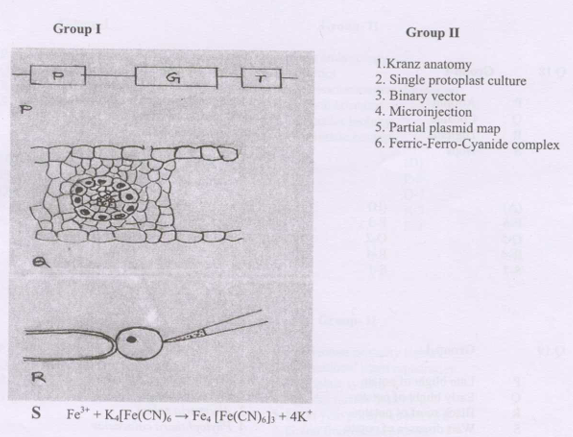
\includegraphics[width=0.9\columnwidth]{FIG/M-16.png}
    \caption*{}
    \label{fig:M-16}
\end{figure}
\begin{multicols}{2}
\begin{enumerate}[label=\Alph*)]
    \item P-3, Q-1, R-4, S-6
    \item P-5, Q-1, R-2, S-3
    \item P-5, Q-1, R-4, S-6
    \item P-3, Q-4, R-1, S-6
\end{enumerate}
\end{multicols}
\item
\begin{multicols}{2}
\textbf{Group-I}
\begin{enumerate}[label=(\Alph*) ,start=16]
    \item Foliaecous bracts
    \item Spathe
    \item Petaloid bracts
    \item Involucre
\end{enumerate}

\columnbreak

\textbf{Group-II}
\begin{enumerate}[label=\arabic*]
    \item A large and commonly boat shaped bract enclosing a cluster of flowers
    \item One or more whorls of bracteoles developing at the base of a calyx
    \item Green, flat and leaf like in appearance
    \item Brightly coloured bracts looking somewhat like petals
    \item Special bracts - small, dry and scaly
    \item One or more whorls of bracts, normally green in colour present around a cluster of flowers
\end{enumerate}
\end{multicols}

\begin{multicols}{2}
\begin{enumerate}[label=(\Alph*)]
    \item P-5 Q-2 R-3 S-4
    \item P-3 Q-1 R-4 S-6
    \item P-3 Q-6 R-3 S-2
    \item P-4 Q-5 R-2 S-1
\end{enumerate}
\end{multicols}

% Q.18
\item
\begin{multicols}{2}
\textbf{Group-I}
\begin{enumerate}[label=(\Alph*) ,start=16]
    \item Atropin
    \item Cocaine
    \item Digitalis
    \item Hops
\end{enumerate}

\columnbreak

\textbf{Group-II}
\begin{enumerate}[label=\arabic*.]
    \item \textit{Digitalis purpurea}
    \item \textit{Triticum aestivum}
    \item \textit{Erythroxylon coca}
    \item \textit{Humulus lupulus}
    \item \textit{Atropa belladonna}
    \item \textit{Datura stramonium}
\end{enumerate}
\end{multicols}

\begin{multicols}{2}
\begin{enumerate}[label=(\Alph*)]
    \item P-6 Q-5 R-4 S-2
    \item P-3 Q-2 R-4 S-1
    \item P-5 Q-3 R-1 S-4
    \item P-6 Q-5 R-3 S-1
\end{enumerate}
\end{multicols}

% Q.19
\item
\begin{multicols}{2}
\textbf{Group-I}
\begin{enumerate}[label=(\Alph*) ,start=16]
    \item Late blight of potato
    \item Early blight of potato
    \item Black scurf of potato
    \item Wart diseases of potato
\end{enumerate}

\columnbreak

\textbf{Group-II}
\begin{enumerate}[label=\arabic*.]
    \item \textit{Synchytrium endobioticum}
    \item \textit{Rhizoctonia solani}
    \item \textit{Alternaria solani}
    \item \textit{Phytophthora colocasiae}
    \item \textit{Phytophthora arecaecae}
    \item \textit{Phytophthora infestans}
\end{enumerate}
\end{multicols}

\begin{multicols}{2}
\begin{enumerate}[label=(\Alph*)]
    \item P-6 Q-3 R-2 S-1
    \item P-6 Q-3 R-2 S-2
    \item P-5 Q-3 R-2 S-1
    \item P-4 Q-3 R-2 S-1
\end{enumerate}
\end{multicols}
\item
\begin{multicols}{2}
\textbf{Group-I}
\begin{enumerate}[label=(\Alph*) ,start=16]
    \item Insect Resistance Rice
    \item Non-antibiotic selection system
    \item Antibiotic marker gene
    \item C4 photosynthesis
\end{enumerate}

\columnbreak

\textbf{Group-II}
\begin{enumerate}[label=\arabic*.]
    \item \textit{psy}
    \item \textit{cryIAb}
    \item \textit{hpt}
    \item PEPC
    \item PMI
    \item Rubisco
\end{enumerate}
\end{multicols}

\begin{multicols}{2}
\begin{enumerate}[label=(\Alph*)]
    \item P-2 Q-1 R-3 S-4
    \item P-5 Q-2 R-1 S-6
    \item P-2 Q-4 R-3 S-5
    \item P-1 Q-2 R-4 S-6
\end{enumerate}
\end{multicols}

% Q.21
\item
\begin{multicols}{2}
\textbf{Group-I}
\begin{enumerate}[label=(\Alph*) ,start=16]
    \item P. Maheshwari
    \item E. Hood
    \item B. McClintock
    \item S. M. Sarkar
\end{enumerate}

\columnbreak

\textbf{Group-II}
\begin{enumerate}[label=\arabic*.]
    \item Plant embryology
    \item Genetics
    \item \textit{Agrobacterium} transformation
    \item Growth hormone
    \item Molecular biology
    \item Systematic botany
\end{enumerate}
\end{multicols}

\begin{multicols}{2}
\begin{enumerate}[label=(\Alph*)]
    \item P-1 Q-6 R-3 S-2
    \item P-1 Q-3 R-2 S-4
    \item P-2 Q-1 R-5 S-5
    \item P-2 Q-1 R-5 S-3
\end{enumerate}
\end{multicols}

% Q.22
\item
\begin{multicols}{2}
\textbf{Group-I}
\begin{enumerate}[label=(\Alph*) ,start=16]
    \item IPR
    \item Selectable reporter gene
    \item Vectorless DNA transfer
    \item Selectable marker gene
\end{enumerate}

\columnbreak

\textbf{Group-II}
\begin{enumerate}[label=\arabic*.]
    \item Intellectual property rights
    \item International plant registration
    \item Protoplast system
    \item \textit{Agrobacterium} system
    \item Neomycin phosphotransferase
    \item Green fluorescent protein
\end{enumerate}
\end{multicols}

\begin{multicols}{2}
\begin{enumerate}[label=(\Alph*)]
    \item P-1 Q-6 R-3 S-5
    \item P-1 Q-6 R-3 S-2
    \item P-2 Q-5 R-4 S-5
    \item P-2 Q-5 R-4 S-6
\end{enumerate}
\end{multicols}
\noindent\textbf{Common Data Questions}  

\noindent\textbf{Common Data for Questions 23 and 24:}

Union of stamens may involve adhesion or cohesion. Arrangement of stamens of a flower is given below:
\begin{figure}[h!]
    \centering
    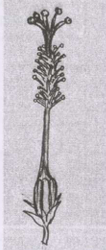
\includegraphics[height=4cm]{FIG/M-24.png}
    \caption*{}
    \label{fig:M-24}
\end{figure}


\item Identify the type of statement 
\begin{multicols}{2}
\begin{enumerate}[label=(\Alph*)]
    \item Diadelphous
    \item Monadelphous
    \item Polyadelphous
    \item Syngenesious
\end{enumerate}
\end{multicols}

% Q24
\item Identify the family from the type of stamens  
\begin{multicols}{2}
\begin{enumerate}[label=(\Alph*)]
    \item Malvaceae
    \item Solanaceae
    \item Compositae
    \item Apiaceae
\end{enumerate}
\end{multicols}


% Linked Answer Questions
\noindent\textbf{Linked Answer Questions: Q.25 to Q.28 carry two marks each.}  

\noindent\textbf{Statement for Linked Answer Questions 25 and 26:}  

The following reaction is taking place in aerobic organisms.

\[
CH_3SCoA +
\chemfig{CH_3SCoA} +
\chemfig{C([::90]=O)([::180]-COO^{-})([::270]=CH_2-COO^{-})}
\overset{k_{2}}{\rightleftharpoons}
\chemfig{C([::90]-OH)([::180]-COO^{-})([::270]=CH_2-COO^{-})([::360]=CH_2-COO^{-})} + 
\chemfig{CoASH}
\]


\item Identify the products from the above reaction  
\begin{multicols}{2}
\begin{enumerate}[label=(\Alph*)]
    \item Isocitrate and Coenzyme A
    \item Citrate and Coenzyme A
    \item Pyruvate and acetyl CoA
    \item Succinate and acetyl CoA
\end{enumerate}
\end{multicols}

% Q26
\item Identify the enzyme and the type of reaction  
\begin{multicols}{2}
\begin{enumerate}[label=(\Alph*)]
    \item Citrate synthase and condensation reaction
    \item Citrate synthetase and condensation reaction
    \item Isocitrate dehydrogenase and oxidative decarboxylation
    \item Aconitase and dehydration reaction
\end{enumerate}
\end{multicols}
\noindent\textbf{Statement for Linked Answer Questions 27 and 28:}  

The visible spectrum of light lies between 400--700 nm. The correlation of expression of wavelength is given below:  

\[
1 \, \text{m} \rightarrow 10^3 \, \text{mm} \rightarrow 10^6 \, \mu\text{m} \rightarrow 10^9 \, \text{nm} \rightarrow 10^{10} \, \text{\AA}
\]

\begin{center}
\begin{tabular}{l l}
\textbf{Colour Spectrum} & \textbf{Wavelength (nm)} \\
P Blue & 1. 500--550 \\
Q Green & 2. 450--500 \\
R Yellow & 3. 650--700 \\
S Red & 4. 550--600 \\
\end{tabular}
\end{center}

\item Identify the correct combination from the above options  
\begin{multicols}{2}
\begin{enumerate}[label=(\Alph*)]
    \item P--1, Q--2, R--4, S--3
    \item P--2, Q--1, R--3, S--4
    \item P--2, Q--1, R--4, S--3
    \item P--3, Q--1, R--2, S--4
\end{enumerate}
\end{multicols}

% Q28
\item For conversion of wavelength from nm to \AA{} and $\mu$m  
\begin{multicols}{2}
\begin{enumerate}[label=(\Alph*)]
    \item Divide the wavelength by 10 and $10^{-3}$
    \item Multiply the wavelength by 10 and $10^{-3}$
    \item Divide the wavelength by 10 and $10^{-4}$
    \item Multiply the wavelength by 10 and $10^{-5}$
\end{enumerate}
\end{multicols}
\begin{center}
\textbf{END OF SECTION - M}
\end{center}
\end{enumerate}
\end{document}
